\documentclass[12pt,a4paper]{article}
\usepackage[utf8]{inputenc}
\usepackage{amsmath}
\usepackage{amsfonts}
\usepackage{amssymb}
\usepackage{graphicx}
\usepackage[left=1.00in, right=1.00in, top=1.00in, bottom=1.00in]{geometry}
\usepackage{fontspec}
%\setmainfont{Times New Roman}

\usepackage{enumerate}
\usepackage{booktabs}
\usepackage{fontspec}
\usepackage{bm}
%minted --insert code
\usepackage{minted}
\usepackage{xcolor}
\definecolor{background-color}{HTML}{f3f3f3} %background-color
\newcommand{\inputmintedfile}[2]{
	\inputminted[linenos=true,
	bgcolor=background-color,
	fontsize= \footnotesize,
	fontfamily=courier ,
	breaklines=true
	]{#1}
	{#2}
}
%algorithm redefine
\usepackage{algorithm}
\usepackage{algorithmicx}
\usepackage{algpseudocode}
\renewcommand{\algorithmicrequire}{\textbf{Input:}}
\renewcommand{\algorithmicensure}{\textbf{Output:}}
\renewcommand{\thesection}{\arabic{section}.} 
\renewcommand{\thesubsection}{\roman{subsection}.}
%tikz plot
\usepackage{tikz}
\usetikzlibrary{arrows.meta, positioning,chains}


\author{Zuyao Chen  201728008629002}
\title{Assignment 5 of Algorithm}
\date{} 



\begin{document}
	\maketitle
\section{Integer Programming}

\textbf{Proof:} \\
\begin{itemize}
	\item Certificate: we can verify the constraints $Ax \geq b $ in polynomial time, thus it is a NP problem;
	\item NP-hard: Now we show that $\text{3-SAT} \leq_{P} \text{Integer Programming}$.
	Let $C_i$($i=1,2,...,m$) be the clauses of 3-SAT problem $\phi = C_1 \wedge C_2 \wedge \cdots \wedge C_m$, $x = (x_1,x_2,...,x_n)$.Once we construct a matrix $A$ and $b$ that each clause $C_i$ can be True or False corresponding to the True or False of the constraint $ a_{i1}x_1 + a_{i2}x_2 + ... + a_{in}x_n \geq b_i$
	, then $\phi$ is satisfied iff $Ax \geq b$ holds. \\
	For instance, $m=3$, $n =4$, $x_i = \{0,1\}$, $\phi =  (x_1 \vee x_2 \vee \neg x_3) \wedge (\neg x_1 \vee x_2 \vee x_4   ) \wedge (x_2 \vee x_3 \vee   x_4)$.  The corresponding constraints are $x_1 + x_2 + (1-x_3) \geq 1$,	$(1-x_1) + x_2 + x_4 \geq 1$ and 
	$ x_2 + x_3 + x_4 \geq 1$,
	we can easily construct the matrix $A$ and $b$ by rewriting the constraints.Thus $3$-SAT is polynomially reducible to the Integer programming. 
\end{itemize}
Hence , the Integer Programming problem is in NP-complete.
\section{Airplane Landing Problem}
 Let $x_1, x_2,...,x_n $ be the exact landing time of each airplane respectively, the problem can be written as 
 \[	\begin{split} 
	 \max  \quad &\min(x_2 - x_1, x_3 - x_2, ..., x_n - x_{n-1}) \\
	 \text{s.t.} \quad & s_1 \leq x_1 \leq t_1 \\
	 & s_2 \leq x_2 \leq t_2  \\
	 &\cdots \\
	 & s_n \leq x_n \leq t_n
	\end{split}  
 \]
 for instance, we have $n = 4, [10,20],[40,60],[75,80],[100,120]$ ( here the minute is the metric of time),
 using tool cvxpy we can obtain the optimal solution $35$ with optimal variables $x_1 = 10, 45,80,116$.
 \begin{figure}[H]
 	\centering
 	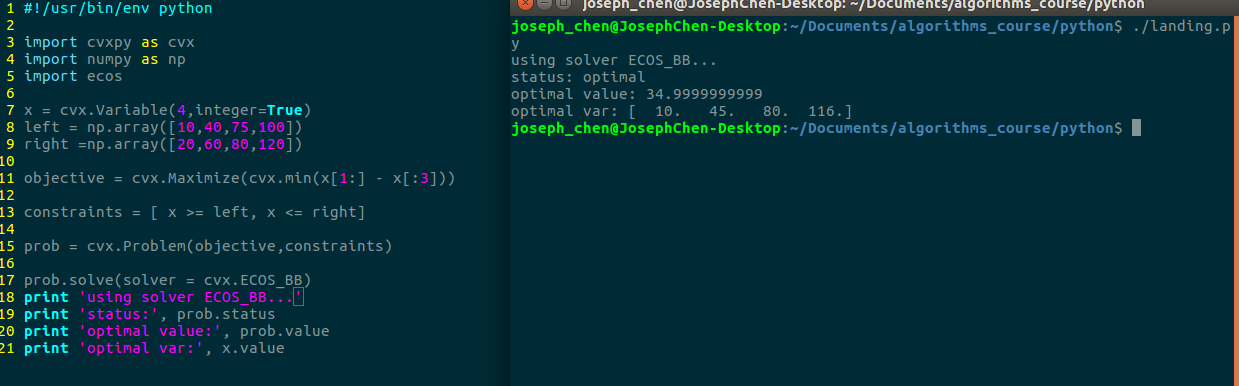
\includegraphics[width=.8\textwidth]{work4/landing}
 \end{figure}
 
\section{Maximum length}
Code is written using C++ in accessory file `max\_length.cpp'.
Here is a test example ,
\begin{figure}[H]
\centering
\includegraphics[width=0.9\textwidth,height=0.06\textheight]{pictures/max} 		
\end{figure}
\section{Ford Fulkerson}
 
\begin{figure}[H]
 \centering 
	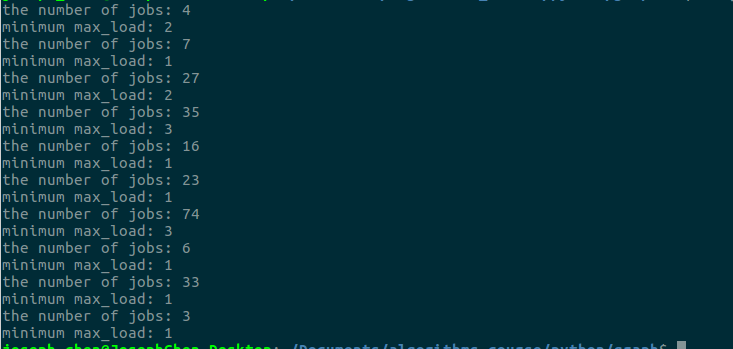
\includegraphics[width = 0.8\textwidth,height = 0.2\textheight]{work5/load_balance}
\end{figure} 	 
\section{Push relabel}
 
\begin{figure}[H]
 \centering 
	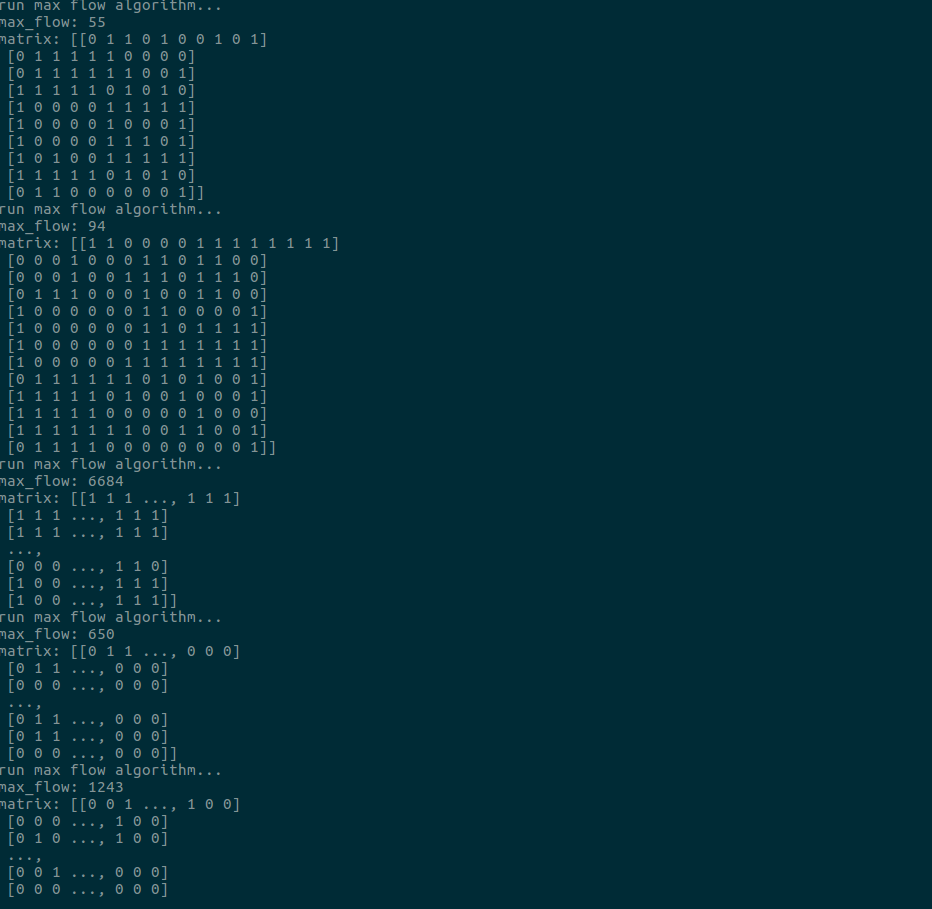
\includegraphics[width = 0.8\textwidth,height = 0.25\textheight]{work5/push1}
\end{figure} 	
the test result on `problem2.data' is showed above,
 the correctness of algorithm can be validated by broute fource.
 It is worth noting that using push relabel insead of Ford Fulkerson 
 is wise since time complexity.
 
 
	
	
\end{document}